\documentclass[11pt,openany]{article}
\usepackage[dutch]{babel}
\usepackage{amsmath}
\usepackage{amssymb}
\usepackage{graphicx}
\usepackage{enumitem}
\usepackage[center]{caption}
\usepackage{a4wide}
\setcounter{tocdepth}{1}
\setlength{\parindent}{0pt}
\usepackage{multirow}
\usepackage{fancyhdr}
\usepackage{blindtext}


\begin{document}
	
	\tableofcontents
	\newpage
	
\section{Introductie}

\subsection{Wat is Solvas Fleet?}
Solvas Fleet is een web based applicatie die instaat voor het beheren van klant- en polisgegevens van een voertuigvloot. Met Solvas Fleet is het mogelijk om ten alle tijde deze gegevens te kunnen beheren zonder daarbij te moeten wachten op informatie of zich te verplaatsen.  Hierbij zal Solvas Fleet steeds een duidelijk overzicht van de gegevens voorzien die u nodig heeft en dit in een beveiligde omgeving.\\

Deze gebruikershandleing heeft als doel de gebruiker een zo aangenaam mogelijke ervaring met Solvas Fleet te garanderen en biedt voldoende informatie om een gebruiker zonder enige voorkennis volledig te kunnen assisteren bij het proces. \\

Elke functionaliteit wordt uitvoerig beschreven en zijn afhankelijk van uw functie.

\subsection{Wat is mogelijk met Solvas Fleet?}
Zoals reeds vermeld, wordt Solvas Fleet gebruikt om klant- en polisgegevens van vloten te beheren. De applicatie laat hierbij toe deze gegevens te raadplegen, of met de nodige rechten, ook te kunnen inbrengen,wijzigen of verwijderen uit het systeem. In deze versie van Solvas Fleet wordt onderstaande functionaliteit ondersteund:


\begin{itemize}[noitemsep]
	\item Ondersteuning voor authenticatie
	\item Ondersteuning voor authorisatie
	\item \textbf{Gebruiker}: aanmaken/wijzigen/verwijderen/lijst weergeven
	\item \textbf{Klant}: aanmaken/wijzigen/verwijderen/lijst weergeven
	\item \textbf{Vloot}: aanmaken/wijzigen/verwijderen/lijst weergeven
	\item \textbf{Voertuig}: aanmaken/wijzigen/verwijderen/lijst weergeven
	\item Lijst van alle vloten van een klant weergeven
	\item Lijst van alle voertuigen van een vloot weergeven
	\item Lijst van alle voertuigen van een bepaald type weergeven
	\item \textbf{Verzekeringswaarborg}: toevoegen/wijzijgen/verwijderen/ details weergeven
	\item Factuur opmaken
	\item Lijst van alle facturen weergeven
	\item Details van een factuur weergeven
\end{itemize}
\newpage
\section{Authorisatie}
\subsection{Inloggen bij Solvas Fleet}
Om in te loggen bij Solvas Fleet, volgt u onderstaande stappen:
\begin{enumerate}
	\item Start de Solvas Fleet applicatie. U ziet het inlogscherm weergegeven in Figuur 1.
	\item Vul uw gebruikersnaam en wachtwoord in
	\item Vervolgens klikt u op de login knop om in te loggen bij Solvas Fleet
	\item Indien u succesvol kon inloggen, krijgt u het startscherm te zien zoals weergegeven in Figuur 2. Dit scherm kan verschillen afhankelijk van uw functie.
	\item Rechtsboven in de bovenbalk ziet u de gekozen taal, uw functie en uw gebruikersnaam.
	\item In het andere geval, krijgt u een foutmelding die aangeeft dat u opnieuw uw gegevens moet in
\end{enumerate}

\subsection{Uitloggen bij Solvas Fleet}
Om uit te loggen bij Solvas Fleet, volgt u onderstaande stappen:
\begin{enumerate}
	\item In de bovenbalk klikt u uw gebruikersnaam aan.
	\item U krijgt nu een menu te zien waarin u de optie 'Afmelden' kan kiezen.
	\item Klik vervolgens de optie 'Afmelden' aan.
	\item Tenslotte komt u opnieuw terecht bij het inlogscherm zoals weergegeven in Figuur 1.
\end{enumerate}

\subsection{Instellen taal}
Om de taal naar keuze in te stellen, volgt u onderstaande stappen:
\begin{enumerate}
	\item Rechts in de bovenbalk klikt u op de taaloptie. Deze optie staat standaard ingesteld op 'Nederlands'.
	\item Vervolgens kiest de taal die u wenst. De hele applicatie wordt weergegeven in de door u
	gekozen taal.
\end{enumerate}

\begin{figure}
	\centering
	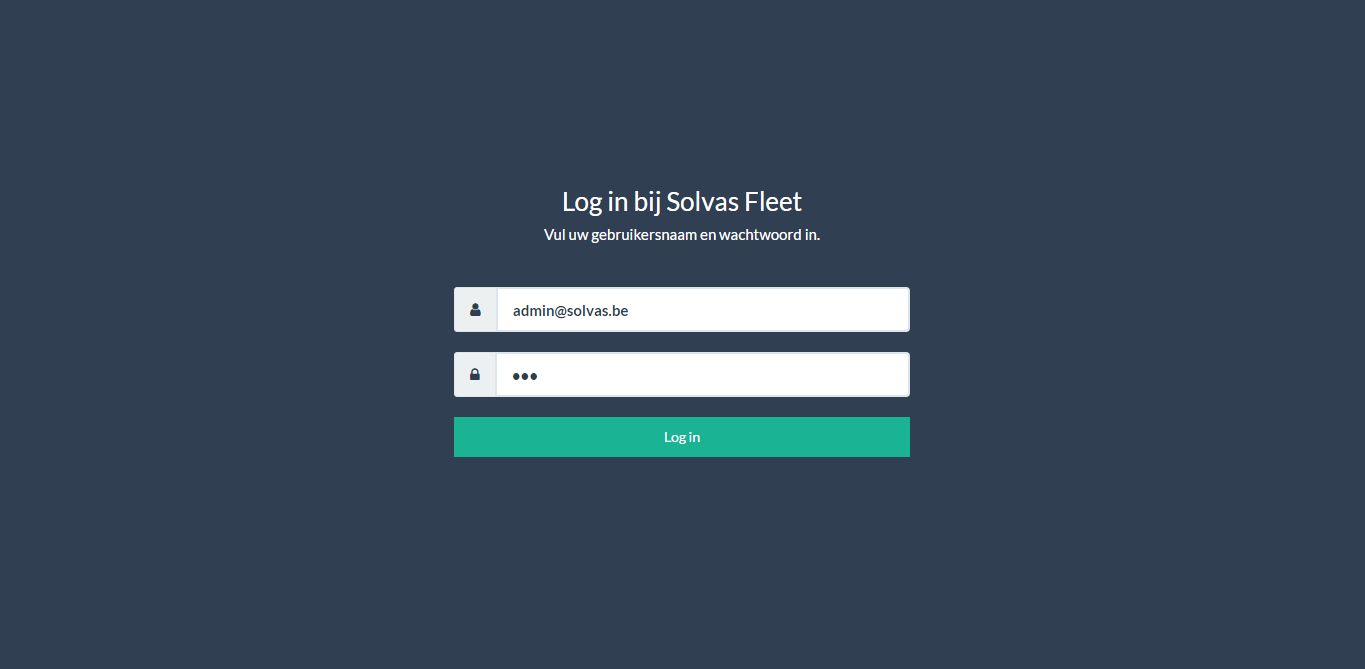
\includegraphics[width=0.9\textwidth]{img/fig_a.png}
	\caption{Inlogscherm Solvas Fleet}
\end{figure}

\begin{figure}
	\centering
	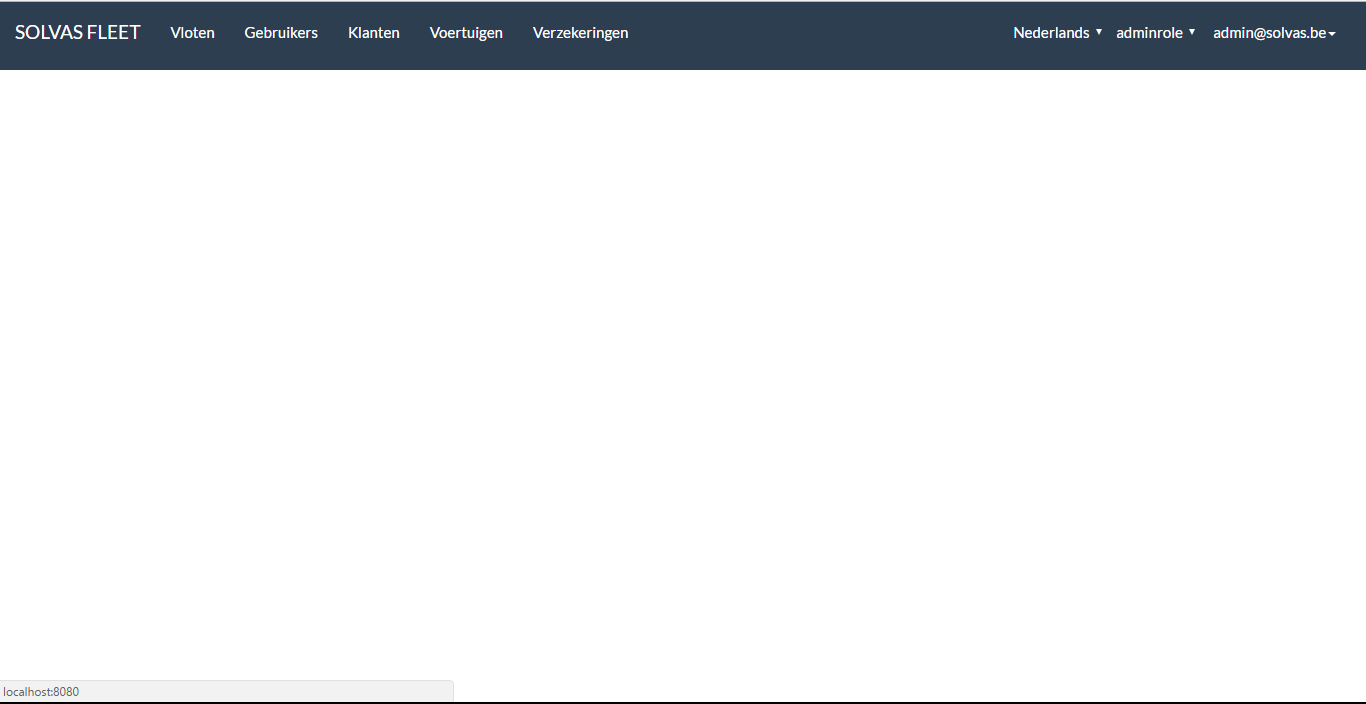
\includegraphics[width=0.9\textwidth]{img/fig_b.png}
	\caption{Startscherm Solvas Fleet (als administrator)}
\end{figure}

\newpage
\section{Gebruiker}
\subsection{Gebruiker aanmaken}

Om een gebruiker aan te maken, volgt u onderstaande stappen:
\begin{enumerate}
	\item Start de Solvas Fleet applicatie en log in. U ziet het startscherm weergegeven in Figuur 2.
	\item In de bovenbalk kiest u voor 'Gebruikers'. U ziet nu een lijst van gebruikers zoals weergegeven in Figuur 3. De weergegeven gebruikers zijn afhankelijk van uw functie.
	\item Om een gebruiker toe te voegen, klikt u op de knop 'Nieuwe gebruiker' bovenaan de pagina. Dit icoon is op Figuur 2 aangeduid in het rood.
	\item U krijgt nu een formulier te zien zoals	 in Figuur 4 met als titel 'Gebruiker aanmaken'.
	\item Vul het formulier op een correcte manier in en bevestig het aanmaken van een gebruiker door de knop 'Gebruiker aanmaken' te klikken (stap 6) of annuleer het proces via de 'Annuleer' knop (stap 7) .
	\item Indien u het aanmaken van een gebruiker bevestigt, komt u opnieuw terecht bij de lijst van gebruikers. 

	\item Indien u het aanmaken van een gebruiker annuleert, komt u opnieuw terecht bij de lijst van gebruikers.
\end{enumerate}
	
	\begin{figure}
		\centering
		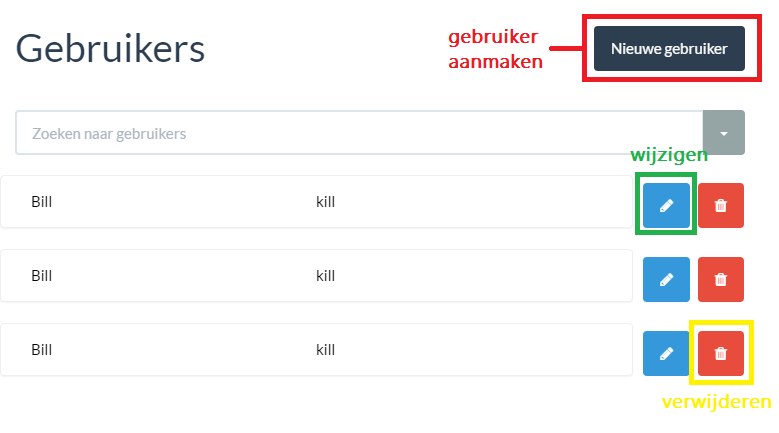
\includegraphics[width=0.9\textwidth]{img/fig_c.png}
		\caption{Lijst van gebruikers}
	\end{figure}

\begin{figure}
	\centering
	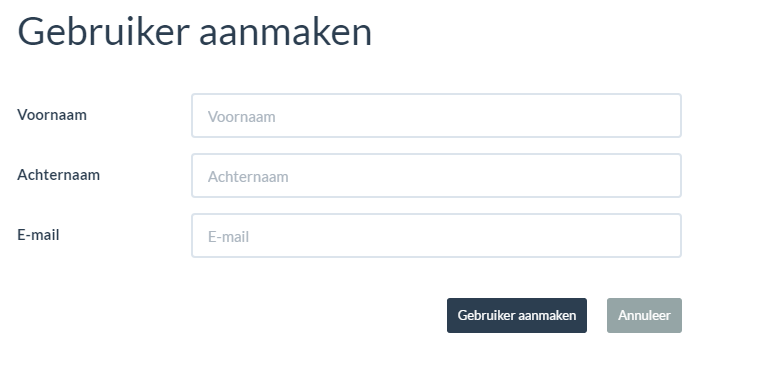
\includegraphics[width=0.9\textwidth]{img/fig_d.png}
	\caption{Aanmaken van gebruiker}
\end{figure}
	
\begin{figure}
	\centering
	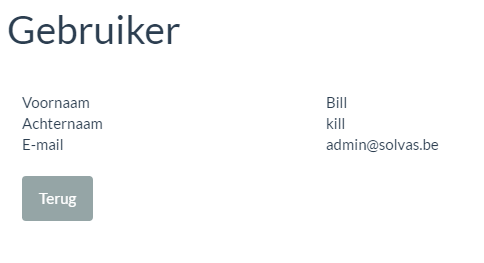
\includegraphics[width=0.9\textwidth]{img/fig_e.png}
	\caption{Informatie gebruiker}
\end{figure}

\newpage
\subsection{Gebruiker wijzigen}

Om een gebruiker te wijzigen, volgt u onderstaande stappen:
\begin{enumerate}
	\item Start de Solvas Fleet applicatie en log in. U ziet het startscherm weergegeven in Figuur 2.
	\item In de bovenbalk kiest u voor 'Gebruikers'. U ziet nu een lijst van alle gebruikers zoals weergegeven in Figuur 3.
	\item Om een gebruiker te wijzigen, klikt u het lichtblauwe penseel icoon aan. Dit icoon is op Figuur 2 aangeduid in het groen.
	\item U krijgt nu een formulier te zien zoals in Figuur 3 met als titel 'Gebruiker aanpassen'.
	\item Vul het formulier op een correcte manier in en en bevestig het wijzigen van een gebruiker door de knop 'Gebruiker bewerken' te klikken (stap 6) of annuleer het proces via de 'Annuleer' knop (stap 7) .
	\item Indien u het wijzigen van een gebruiker bevestigt, komt u opnieuw terecht bij de lijst van gebruikers.
	\item Indien u het wijzigen van een gebruiker annuleert, komt u opnieuw terecht bij de lijst van gebruikers 
\end{enumerate}

\subsection{Gebruiker verwijderen}


Om een gebruiker te verwijderen, volgt u onderstaande stappen:
\begin{enumerate}
	\item Start de Solvas Fleet applicatie en log in. U ziet het startscherm weergegeven in Figuur 2.
	\item In de bovenbalk kiest u voor 'Gebruikers'. U ziet nu een lijst van alle gebruikers zoals weergegeven in Figuur 3.
	\item Om een gebruiker te verwijderen, klikt u op het rode vuilbak icoon. Dit icoon is op Figuur 2 aangeduid in het geel.
	\item De applicatie vraagt om een extra bevestiging. Indien u wilt doorgaan met het verwijderen, kiest u voor 'Ja'. In het andere geval kiest u voor 'Nee'.
	\item Het systeem verwijdert de door u gekozen gebruiker en u bevindt zich opnieuw naar de lijst van gebruikers (Figuur 3).
\end{enumerate}
\newpage
\subsection{Lijst van alle gebruikers weergeven}


Om een lijst van gebruikers te verkrijgen, volgt u onderstaande stappen:
\begin{enumerate}
		\item Start de Solvas Fleet applicatie en log in. U ziet het startscherm weergegeven in Figuur 1.
		\item In de bovenbalk kiest u voor 'Gebruikers'. U ziet nu een lijst van alle gebruikers zoals weergegeven in Figuur 3.
		\item Indien u meer informatie wenst over een gebruiker, klikt u op de desgewenste gebruiker. 
		\item U ziet nu informatie over de gekozen gebruiker zoals weergegeven in Figuur 4. 
		\item Indien u wenst terug te keren naar de lijst van gebruikers, klikt u de knop 'Terug' aan.
\end{enumerate}


\newpage

\section{Klant}
\subsection{Klant aanmaken}

Om een klant aan te maken, volgt u onderstaande stappen:
\begin{enumerate}
	\item Start de Solvas Fleet applicatie en log in. U ziet het startscherm weergegeven in Figuur 2.
	\item In de bovenbalk kiest u voor 'Klanten'. U ziet nu een lijst van klanten zoals weergegeven in Figuur 6. De weergegeven klanten zijn afhankelijk van uw functie.
	\item Om een klant toe te voegen, klikt u op de knop 'Nieuwe klant' bovenaan de pagina. Dit icoon is op Figuur 2 aangeduid in het rood.
	\item U krijgt nu een formulier te zien zoals	 in Figuur 7 met als titel 'Klant aanmaken'.
	\item Vul het formulier op een correcte manier in en bevestig het aanmaken van een klant door de knop 'Klant aanmaken' te klikken (stap 6) of annuleer het proces via de 'Annuleer' knop (stap 7) .
	\item Indien u het aanmaken van een klant bevestigt, komt u opnieuw terecht bij de lijst van klanten. 
	
	\item Indien u het aanmaken van een klant annuleert, komt u opnieuw terecht bij de lijst van 
	klanten.
\end{enumerate}
\begin{figure}
	\centering
	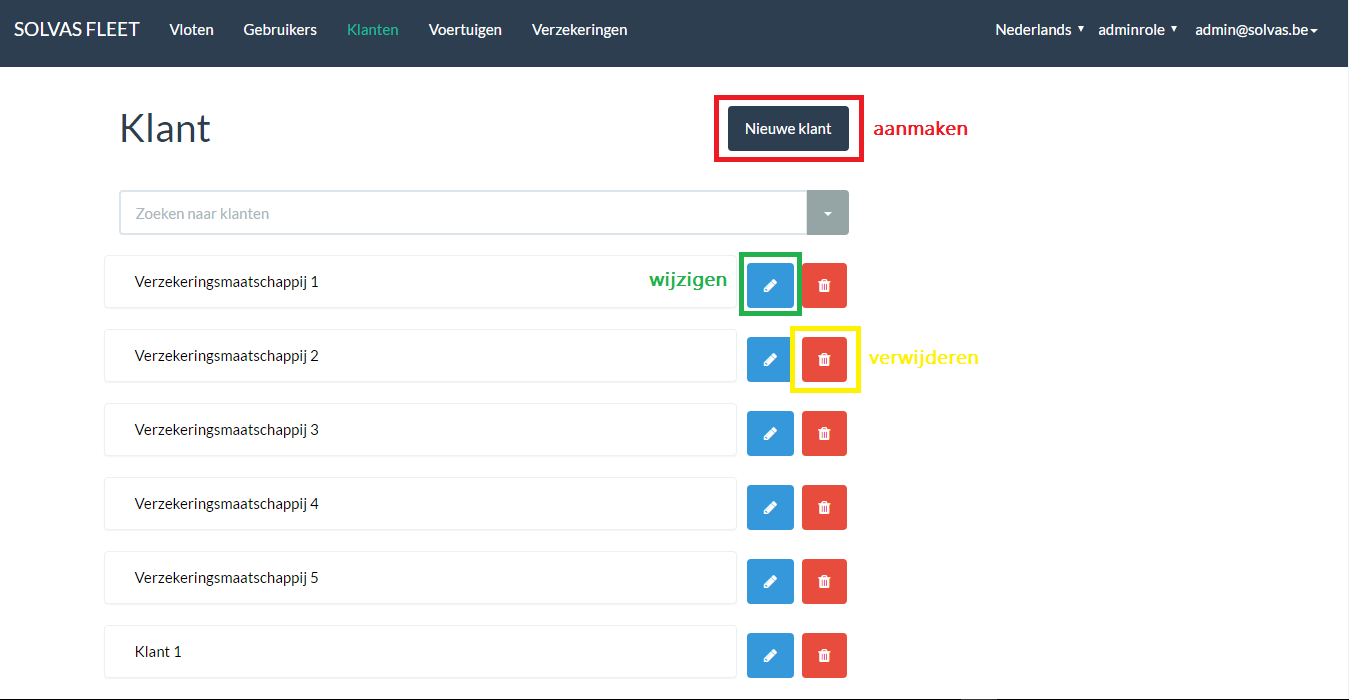
\includegraphics[width=0.9\textwidth]{img/fig_f.png}
	\caption{Lijst van klanten}
\end{figure}

\begin{figure}
	\centering
	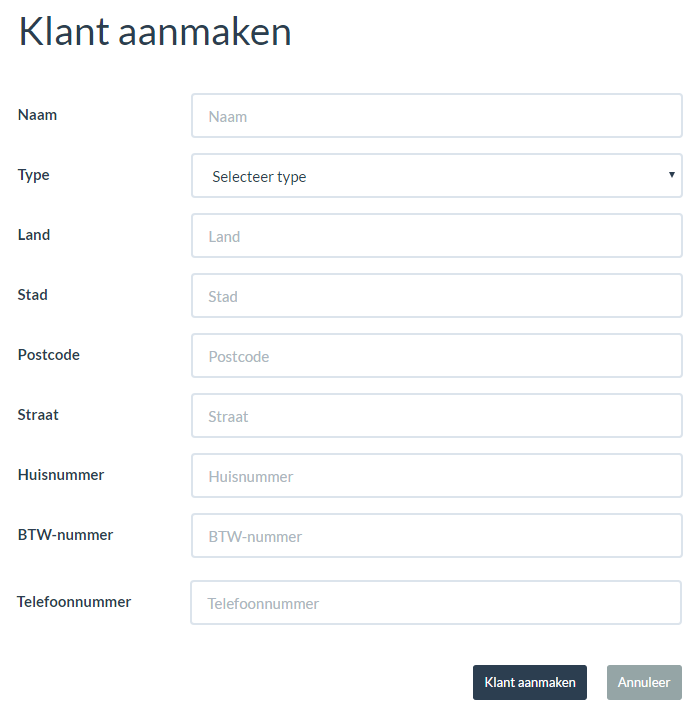
\includegraphics[width=0.9\textwidth]{img/fig_g.png}
	\caption{Formulier klanten}
\end{figure}
\newpage
\subsection{Klant wijzigen}
Om een klant te wijzigen, volgt u onderstaande stappen:
\begin{enumerate}
	\item Start de Solvas Fleet applicatie en log in. U ziet het startscherm weergegeven in Figuur 2.
	\item In de bovenbalk kiest u voor 'Klanten'. U ziet nu een lijst van alle klanten zoals weergegeven in Figuur 6.
	\item Om een klant te wijzigen, klikt u het lichtblauwe penseel icoon aan. Dit icoon is op Figuur 6 aangeduid in het groen.
	\item U krijgt nu een formulier te zien zoals in Figuur 7 met als titel 'Klant aanpassen'.
	\item Vul het formulier op een correcte manier in en en bevestig het wijzigen van een klant door de knop 'Klant bewerken' te klikken (stap 6) of annuleer het proces via de 'Annuleer' knop (stap 7) .
	\item Indien u het wijzigen van een klant bevestigt, komt u opnieuw terecht bij de lijst van klanten.
	\item Indien u het wijzigen van een klant annuleert, komt u opnieuw terecht bij de lijst van klanten 
\end{enumerate}

\subsection{Klant verwijderen}
Om een klant te verwijderen, volgt u onderstaande stappen:
\begin{enumerate}
	\item Start de Solvas Fleet applicatie en log in. U ziet het startscherm weergegeven in Figuur 2.
	\item In de bovenbalk kiest u voor 'Klanten'. U ziet nu een lijst van alle klanten zoals weergegeven in Figuur 6.
	\item Om een klant te verwijderen, klikt u op het rode vuilbak icoon. Dit icoon is op Figuur 6 aangeduid in het geel.
	\item De applicatie vraagt om een extra bevestiging. Indien u wilt doorgaan met het verwijderen, kiest u voor 'Ja'. In het andere geval kiest u voor 'Nee'.
	\item Het systeem verwijdert de door u gekozen klant en u bevindt zich opnieuw naar de lijst van klanten (Figuur 6).
\end{enumerate}

\subsection{Lijst van alle klanten weergeven}
Om een lijst van klanten te verkrijgen, volgt u onderstaande stappen:
\begin{enumerate}
	\item Start de Solvas Fleet applicatie en log in. U ziet het startscherm weergegeven in Figuur 1.
	\item In de bovenbalk kiest u voor 'Klanten'. U ziet nu een lijst van alle klanten zoals weergegeven in Figuur 6.
	\item Indien u meer informatie wenst over een klant, klikt u op de desgewenste klant. 
	\item U ziet nu informatie over de gekozen klant zoals weergegeven in Figuur 8. 
	\item Indien u wenst terug te keren naar de lijst van klanten, klikt u de knop 'Terug' aan.
\end{enumerate}

\begin{figure}
	\centering
	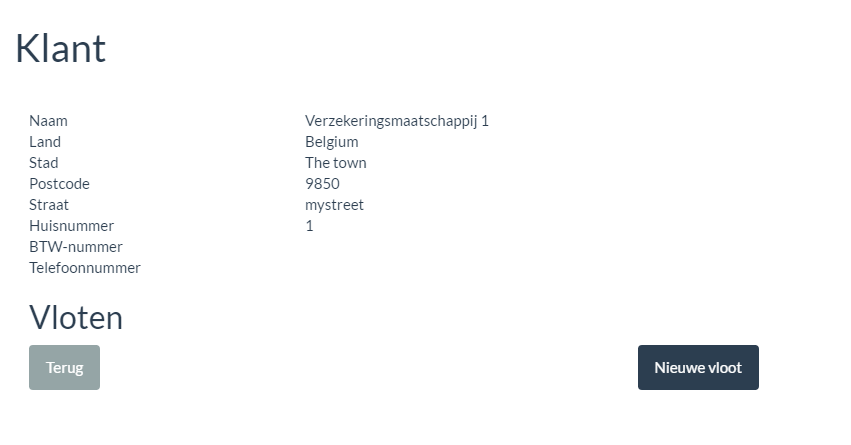
\includegraphics[width=0.9\textwidth]{img/fig_h.png}
	\caption{Informatie over klant}
\end{figure}
\newpage
\section{Vloot}
\subsection{Vloot van een klant aanmaken}
Om een vloot voor een klant aan te maken, volgt u onderstaande stappen:
\begin{enumerate}
	\item Start de Solvas Fleet applicatieen log in. U ziet het startscherm weergegeven in Figuur 2.
	\item In de bovenbalk kiest u voor 'Vloten'. U ziet nu een lijst van alle vloten van de klant zoals weergegeven in Figuur 9.
	\item Om een vloot toe te voegen, klikt u op de knop 'Nieuwe Vloot' bovenaan de pagina. Dit icoon is op Figuur 9 aangeduid in het rood.
	\item U krijgt nu een formulier te zien zoals in Figuur 10 met als titel 'Vloot aanmaken'.
	\item Vul het formulier op een correcte manier in en en bevestig het aanmaken van een vloot door de knop 'Vloot aanmaken' te klikken (stap 6) of annuleer het proces via de 'Annuleer' knop (stap 7) .
	\item Indien u het aanmaken van een vloot bevestigt, komt u opnieuw terecht bij de lijst van vloten.
	\item Indien u het aanmaken van een vloot annuleert, komt u opnieuw terecht bij de lijst van vloten. 
\end{enumerate}

\begin{figure}
	\centering
	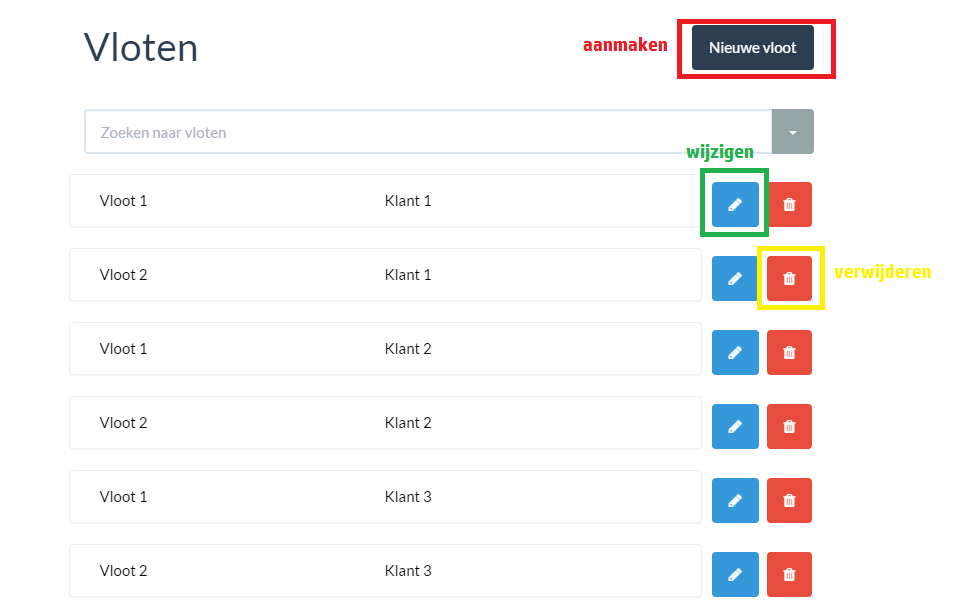
\includegraphics[width=0.9\textwidth]{img/fig_i.png}
	\caption{Lijst van vloten}
\end{figure}

\begin{figure}
	\centering
	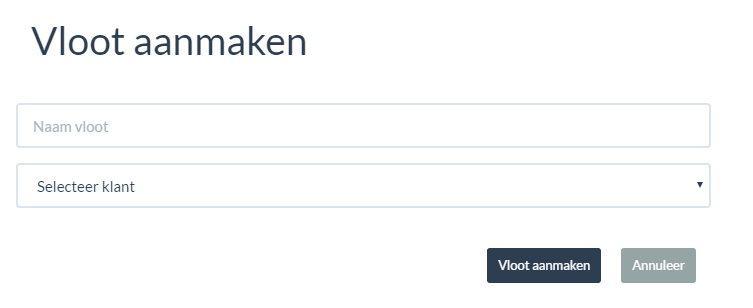
\includegraphics[width=0.9\textwidth]{img/fig_j.png}
	\caption{Formulier vloot}
\end{figure}
\newpage

\subsection{Vloot wijzigen}
Om een vloot te wijzigen, volgt u onderstaande stappen:
\begin{enumerate}
	\item Start de Solvas Fleet applicatie en log in. U ziet het startscherm weergegeven in Figuur 2.
	\item In de bovenbalk kiest u voor 'Vloten'. U ziet nu een lijst van alle vloten van de klant zoals weergegeven in Figuur 8.
	\item Om een vloot te wijzigen, klikt u op het lichtblauwe penseel icoon. Dit is op Figuur 9 aangeduid in het groen
	\item U krijgt nu een formulier te zien zoals in Figuur 10 met als titel 'Vloot bewerken'.
	\item Vul het formulier op een correcte manier in en en bevestig het wijzigen van een vloot door de knop 'Vloot wijzigen' te klikken (stap 6) of annuleer het proces via de 'Annuleer' knop (stap 7) .
	\item Indien u het wijzigen van een vloot bevestigt, komt u opnieuw terecht bij de lijst van vloten.
	\item Indien u het wijzigen van een vloot annuleert, komt u opnieuw terecht bij de lijst van vloten. 
\end{enumerate}

\subsection{Vloot verwijderen}
Om een Vloot te verwijderen, volgt u onderstaande stappen:
\begin{enumerate}
	\item Start de Solvas Fleet applicatie en log in. U ziet het startscherm weergegeven in Figuur 2.
	\item In de bovenbalk kiest u voor 'Vloten'. U ziet nu een lijst van alle vloten zoals weergegeven in Figuur 9.
	\item Om een vloot te verwijderen, klikt u op het rode vuilbak icoon. Dit icoon is op Figuur 9 aangeduid in het geel.
	\item Het systeem verwijdert de door u gekozen vloot en u bevindt zicht opnieuw naar de lijst van vloten (Figuur 9).
\end{enumerate}

\subsection{Lijst van alle vloten van een klant weergeven}
Om een lijst van vloten te verkrijgen, volgt u onderstaande stappen:
\begin{enumerate}
	\item Start de Solvas Fleet applicatie en log in. U ziet het startscherm weergegeven in Figuur 2.
	\item In de bovenbalk kiest u voor 'Vloten'. U ziet nu een lijst van alle vloten van een klant zoals weergegeven in Figuur 9.
	\item Indien u meer informatie wenst over een vloot, klikt u op de desgewenste vloot. 
	\item U ziet nu informatie over de gekozen vloot (afhankelijk van type voertuigen)
	ongeveer zoals weergegeven in Figuur 11. Voor de verdere functionaliteit van deze pagina zie sectie 6 over Voertuigen. 
	\item Indien u wenst terug te keren naar de lijst van vloten, klikt u de knop 'Terug' aan.
\end{enumerate}

\begin{figure}
	\centering
	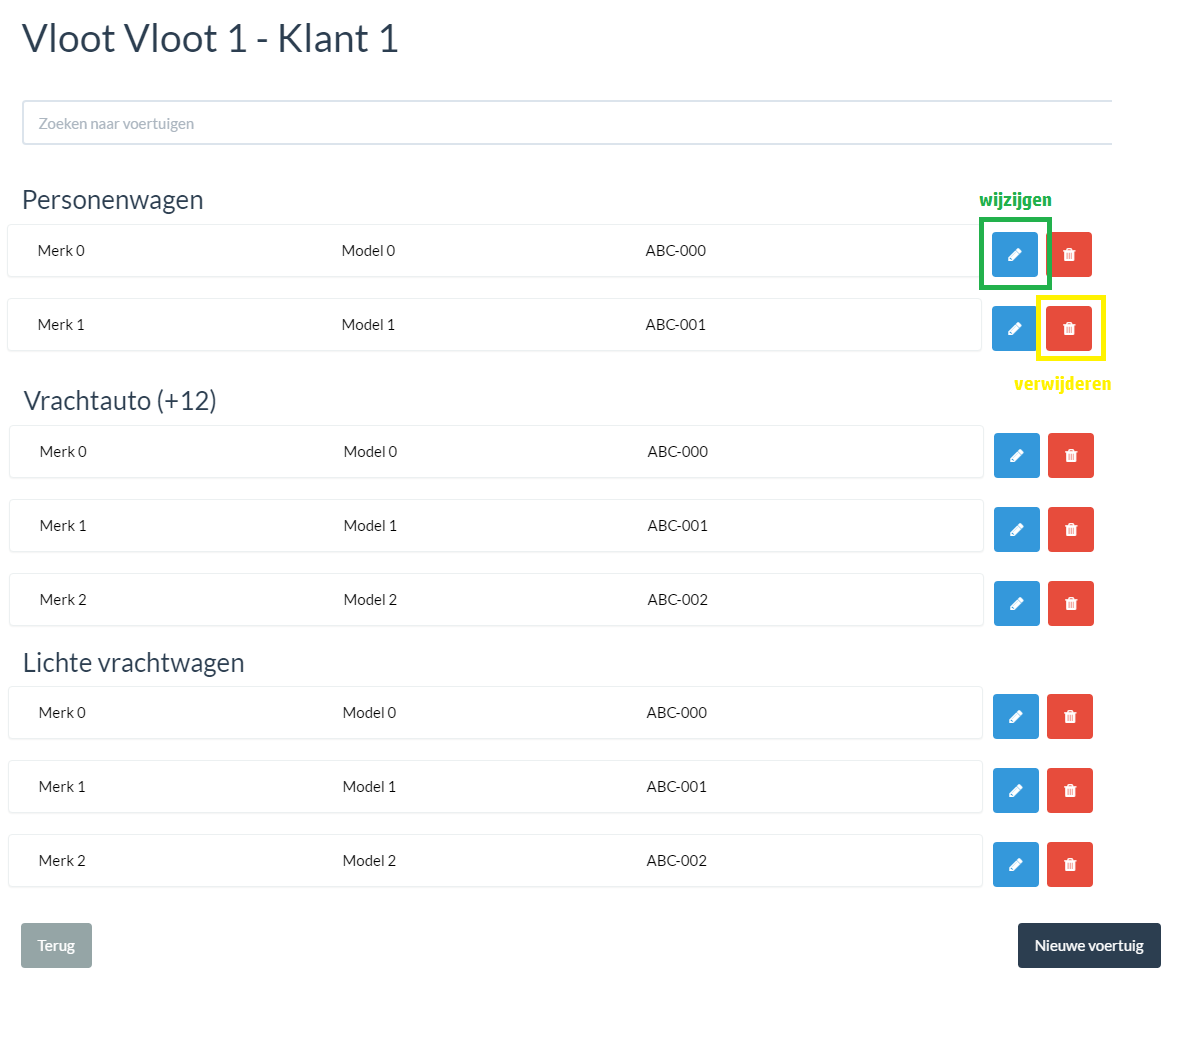
\includegraphics[width=0.9\textwidth]{img/fig_k.png}
	\caption{Informatie over vloot}
\end{figure}

\newpage
\section{Voertuig}
\subsection{Voertuig aanmaken}
Om een voertuig voor een vloot aan te maken, volgt u onderstaande stappen:
\begin{enumerate}
	\item Start de Solvas Fleet applicatie en log in. U ziet het startscherm weergegeven in Figuur 2.
	\item In de bovenbalk kiest u voor 'Vloten'. U ziet nu een lijst van alle vloten van de klant zoals weergegeven in Figuur 9.
	\item Om een voertuig toe te voegen, klikt u op de gewenste vloot waarvoor u een nieuw voertuig wilt toevoegen. 
	\item U krijgt nu een pagina te zien met de informatie (subvloten en voertuigen) van de gekozen vloot
	ongeveer zoals weergegeven in Figuur 11. 
	\item Om een voertuig toe te voegen klikt u onderaan de knop 'Nieuw Voertuig' aan.
	\item U krijgt nu een formulier te zien zoals in Figuur 12 met als titel 'Voertuig aanmaken'.
	\item Vul het formulier op een correcte manier in en bevestig het aanmaken van een voertuig door de knop 'Voertuig aanmaken' aan te klikken (stap 6) of annuleer het proces via de knop 'Annuleer' (stap 7) .
	\item Indien u het aanmaken van een voertuig bevestigt, komt u terecht op de informatiepagina van de vloot zoals weergegeven in Figuur 11. 
	\item Indien u het aanmaken van een voertuig annuleert, komt u opnieuw terecht bij de informatiepagina over de vloot.
\end{enumerate}


\begin{figure}
	\centering
	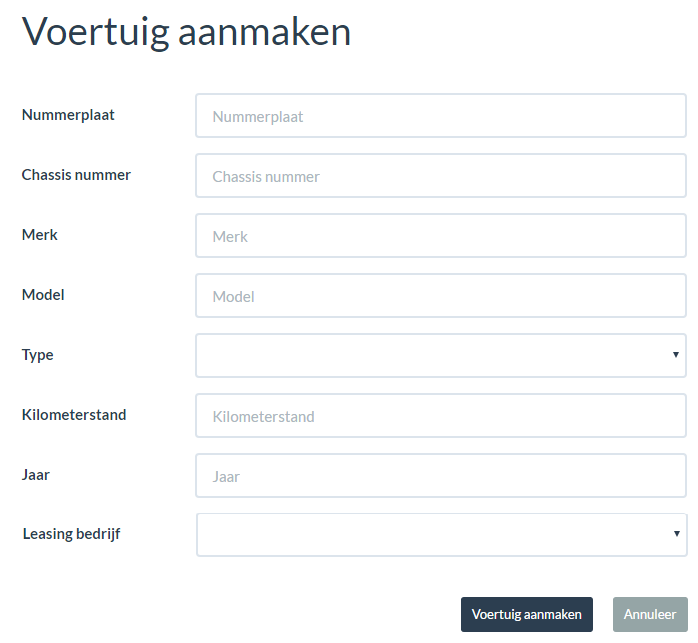
\includegraphics[width=0.9\textwidth]{img/fig_l.png}
	\caption{Formulier voertuig}
\end{figure}

\subsection{Voertuig wijzigen}
Om een voertuig voor een vloot te wijzigen, volgt u onderstaande stappen:
\begin{enumerate}
	\item Start de Solvas Fleet applicatie en log in. U ziet het startscherm weergegeven in Figuur 2.
	\item In de bovenbalk kiest u voor 'Vloten'. U ziet nu een lijst van alle vloten van de klant zoals weergegeven in Figuur 11.
	\item Om een voertuig te wijzigen, klikt u op de gewenste vloot waarvoor u een voertuig wilt wijzigen. 
	\item U krijgt nu een pagina te zien met de informatie (subvloten en voertuigen) van de gekozen vloot
	ongeveer zoals weergegeven in Figuur 11. 
	\item Om een voertuig te wijzigen klikt u op het lichtblauwe penseel icoon. Dit is op Figuur 11 aangeduid in het groen.
	\item U krijgt nu een formulier te zien zoals in Figuur 11 met als titel 'Voertuig bewerken'.
	\item Vul het formulier op een correcte manier in en bevestig het wijzigen van een voertuig door de knop 'Voertuig bewerken' aan te klikken (stap 6) of annuleer het proces via de knop 'Annuleer' (stap 7) .
	\item Indien u het wijzigen van een voertuig bevestigt, komt u terecht op de informatiepagina van de vloot zoals weergegeven in Figuur 11. 
	\item Indien u het wijzgen van een voertuig annuleert, komt u opnieuw terecht bij de informatiepagina over de vloot.
\end{enumerate}

\subsection{Voertuig verwijderen}
Om een voertuig voor een vloot te verwijderen, volgt u onderstaande stappen:
\begin{enumerate}
	\item Start de Solvas Fleet applicatie en log in. U ziet het startscherm weergegeven in Figuur 1.
	\item In de bovenbalk kiest u voor 'Vloten'. U ziet nu een lijst van alle vloten van de klant zoals weergegeven in Figuur 11.
	\item Om een voertuig te verwijderen, klikt u op de gewenste vloot waarvoor u een voertuig wilt verwijderen. 
	\item U krijgt nu een pagina te zien met de informatie (subvloten en voertuigen) van de gekozen vloot
	ongeveer zoals weergegeven in Figuur 11. 
	\item Om een voertuig te wijzigen klikt u op het rode vuilbak icoon. Dit is op Figuur 11 aangeduid in het geel.
	\item Het systeem verwijdert het door u gekozen voertuig en u bevindt zicht opnieuw naar de informatiepagina van uw vloot.
\end{enumerate}


\subsection{Lijst van alle voertuigen (van een bepaald type) van een vloot weergeven}
\begin{enumerate}
	\item Start de Solvas Fleet applicatie en log in. U ziet het startscherm weergegeven in Figuur 2.
	\item In de bovenbalk kiest u voor 'Vloten'. U ziet nu een lijst van alle vloten van de klant zoals weergegeven in Figuur 11.
	\item Om een lijst van voertuigen te verkrijgen, klikt u op de gewenste vloot.
	\item U krijgt nu een pagina te zien met de informatie (subvloten en voertuigen) van de gekozen vloot
	ongeveer zoals weergegeven in Figuur 11. Hier ziet u alle voertuigen die bij deze vloot horen onderverdeeld in subvloten per voertuigtype.
\end{enumerate}

\subsection{Voertuigen zoeken}
Om een voertuig te zoeken, volgt u onderstaande stappen:
\begin{enumerate}
	\item Start de Solvas Fleet applicatie en log in. U ziet het startscherm weergegeven in Figuur 2.
	\item In de bovenbalk kiest u voor 'Voertuigen'. U ziet nu een zoekoptie zoals weergegeven in Figuur 13.
	\item Om een lijst van voertuigen te verkrijgen, vult u de velden in waarnaar u wilt zoeken en klikt u het zoekicoon aan.
	\item U krijgt de voertuigen te zien die aan uw zoekopdracht voldoet ongeveer zoals weergegeven in Figuur 14.
	\item Van hieruit kan u nu alle functies uitvoeren op voertuigen zoals beschreven in sectie 6.
\end{enumerate}

\begin{figure}
	\centering
	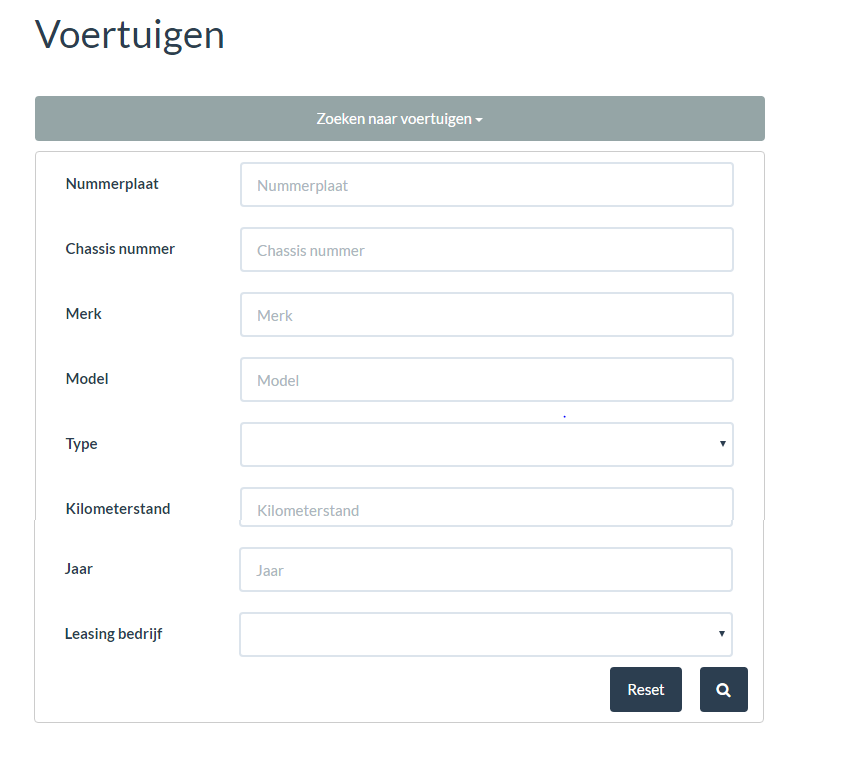
\includegraphics[width=0.9\textwidth]{img/fig_m.png}
	\caption{Zoeken naar voertuig()}
\end{figure}

\begin{figure}
	\centering
	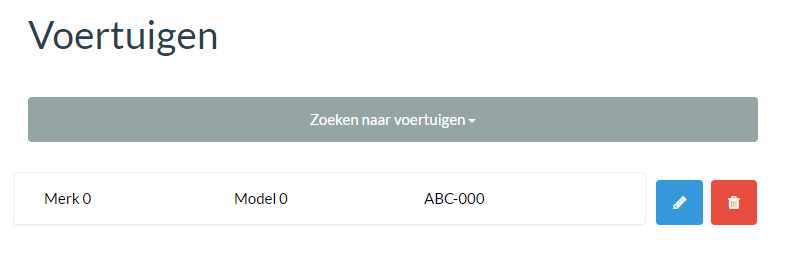
\includegraphics[width=0.9\textwidth]{img/fig_n.png}
	\caption{Resultaat zoeken naar voertuig(en)}
\end{figure}

\section{Verzekeringen}
\subsection{Lijst van verzekeringscontracten weergeven}
Om een lijst van verzekeringscontracten weer te geven, volgt u onderstaande stappen:
\begin{enumerate}
	\item Start de Solvas Fleet applicatie en log in. U ziet het startscherm weergegeven in Figuur 2.
	\item In de bovenbalk kiest u voor 'Verzekeringen'. U ziet nu een lijst van verzekeringscontracten zoals weergegeven in Figuur 15.
	\item Om de verzekeringswaarborgen van een contract te bekijken klikt u een verzekeringscontract aan. Dit is op Figuur 15 aangeduid in het paars.
	\item U krijgt nu de verzekeringswaarborgen van het contract te zien zoals weergegeven in Figuur 16.
\end{enumerate}

\subsection{Verzekeringswaarborg toevoegen}
Om een verzekeringswaarborg toe te voegen, volgt u onderstaande stappen:
\begin{enumerate}
	\item Volg de actie 'Lijst van verzekeringscontracten weergeven'. U krijgt nu een scherm te zien ongeveer weergegeven zoals Figuur 16.
	\item Om een verzekeringswaarborg toe te voegen klikt u de knop 'Nieuwe verzekeringswaarborg' aan.
	\item U krijgt een scherm te zien zoals weergegeven in Figuur 17.
	\item Vul het formulier op een correcte manier in, en bevestig het aanmaken via 'Verzekering aanmaken' of annuleer via 'Annuleer'
\end{enumerate}
\subsection{Verzekeringswaarborg wijzigen}
Om een verzekeringswaarborg toe te wijzigen, volgt u onderstaande stappen:
\begin{enumerate}
	\item Volg de actie 'Lijst van verzekeringscontracten weergeven'. U krijgt nu een scherm te zien ongeveer weergegeven zoals Figuur 16.
	\item Om een verzekeringswaarborg toe te wijzgen klikt u de knop het blauwe penseel icoon aan naast de verzekeringswaarborg.
	\item U krijgt een scherm te zien zoals weergegeven in Figuur 17.
	\item Vul het formulier op een correcte manier in, en bevestig het wijzigen via 'Verzekering bewerken' of annuleer via 'Annuleer'
\end{enumerate}

\subsection{Verzekeringswaarborg verwijderen}
Om een verzekeringswaarborg toe te verwijderen, volgt u onderstaande stappen:
\begin{enumerate}
	\item Volg de actie 'Lijst van verzekeringscontracten weergeven'. U krijgt nu een scherm te zien ongeveer weergegeven zoals Figuur 16.
	\item Om een verzekeringswaarborg toe te verwijderen klikt het rode vuilbak icoon aan naast de verzekeringswaarborg.
\end{enumerate}
\subsection{Verzekeringswaarborg bekijken}
	Om een verzekeringswaarborg te bekijken, volgt u onderstaande stappen:
	\begin{enumerate}
		\item Volg de actie 'Lijst van verzekeringscontracten weergeven'. U krijgt nu een scherm te zien ongeveer weergegeven zoals Figuur 16.
		\item Om een verzekeringswaarborg te bekijken, klikt u de verzekeringswaarborg aan. 
		\item U krijgt nu een scherm te zien ongeveer zoals weergegeven in Figuur 18.
	\end{enumerate}

\begin{figure}
	\centering
	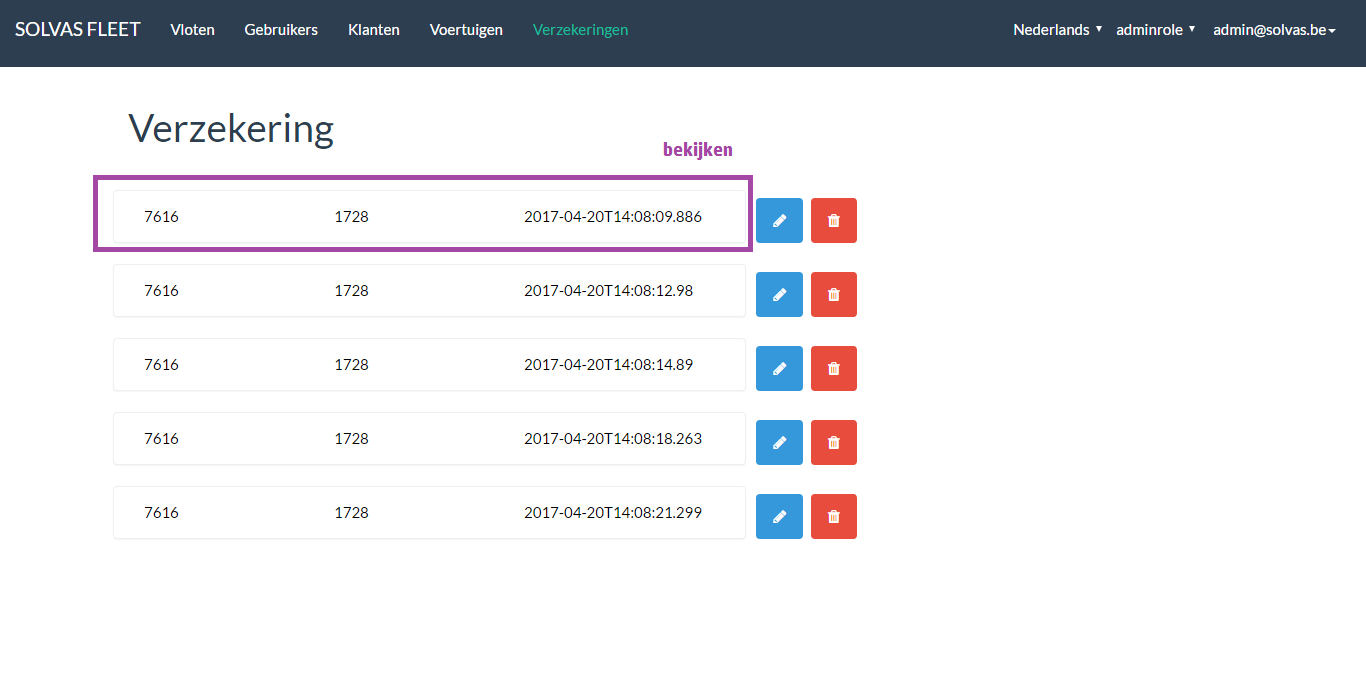
\includegraphics[width=0.9\textwidth]{img/fig_o.png}
	\caption{Lijst van verzekeringscontracten}
\end{figure}

\begin{figure}
	\centering
	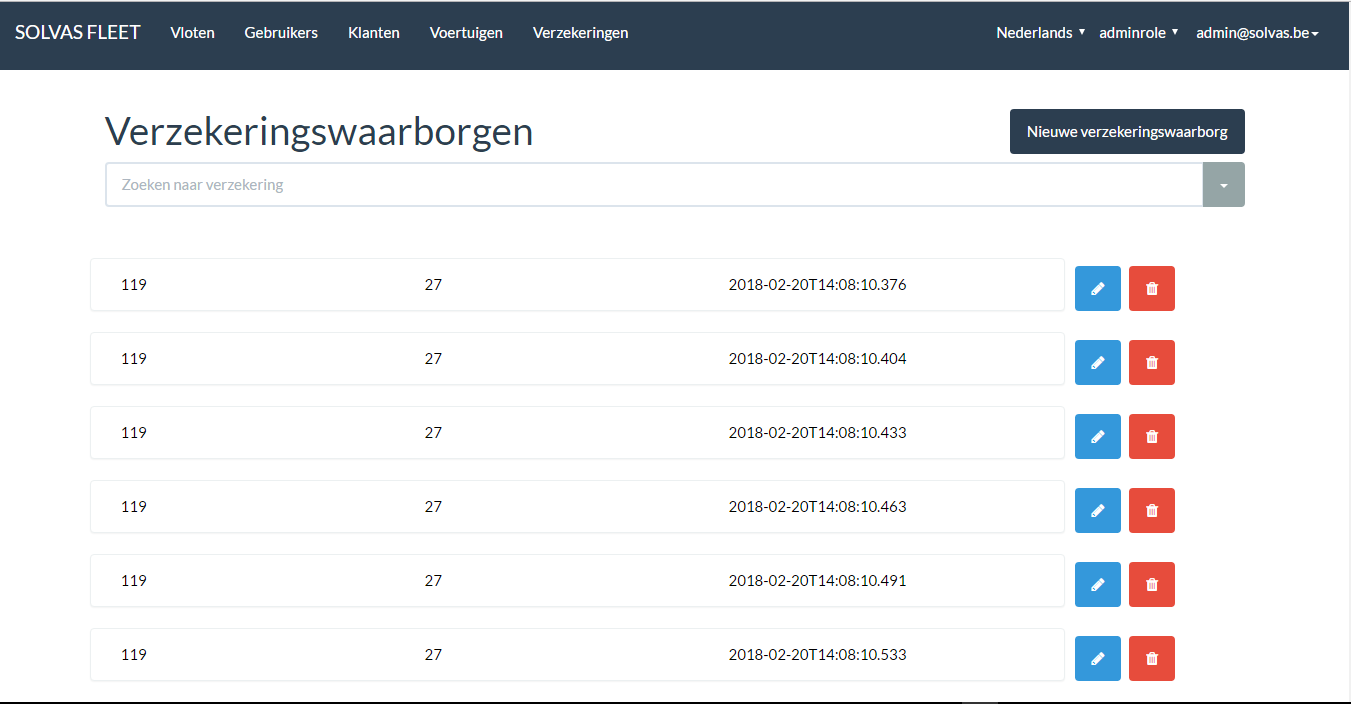
\includegraphics[width=0.9\textwidth]{img/fig_p.png}
	\caption{Lijst van verzekeringswaarborgen}
\end{figure}

\begin{figure}
	\centering
	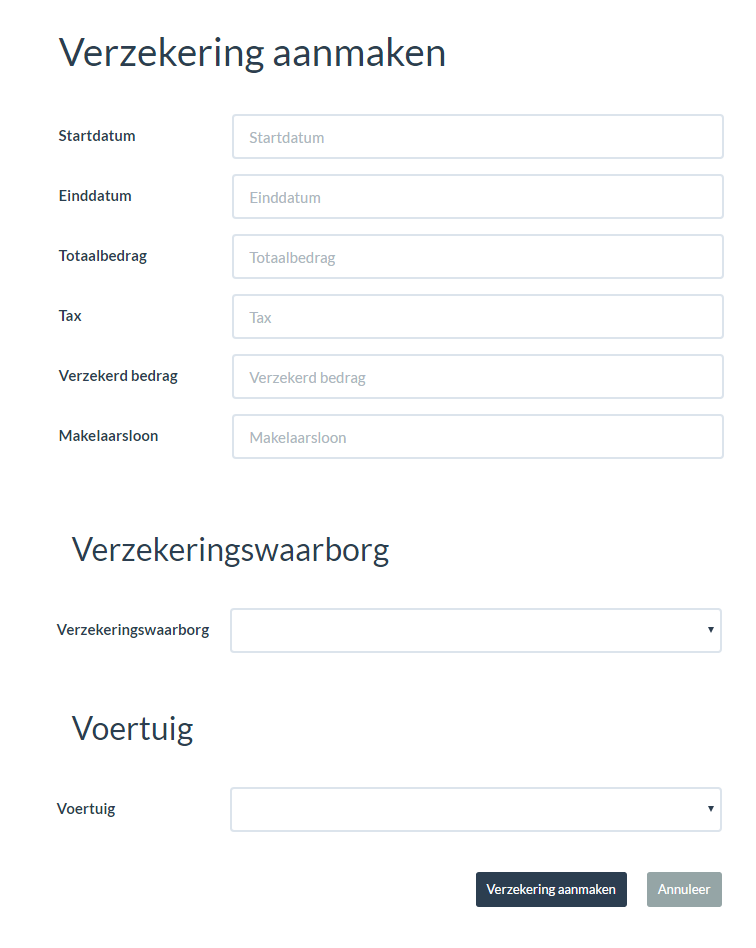
\includegraphics[width=0.9\textwidth]{img/fig_q.png}
	\caption{Formulier verzekeringswaarborg}
\end{figure}

\begin{figure}
	\centering
	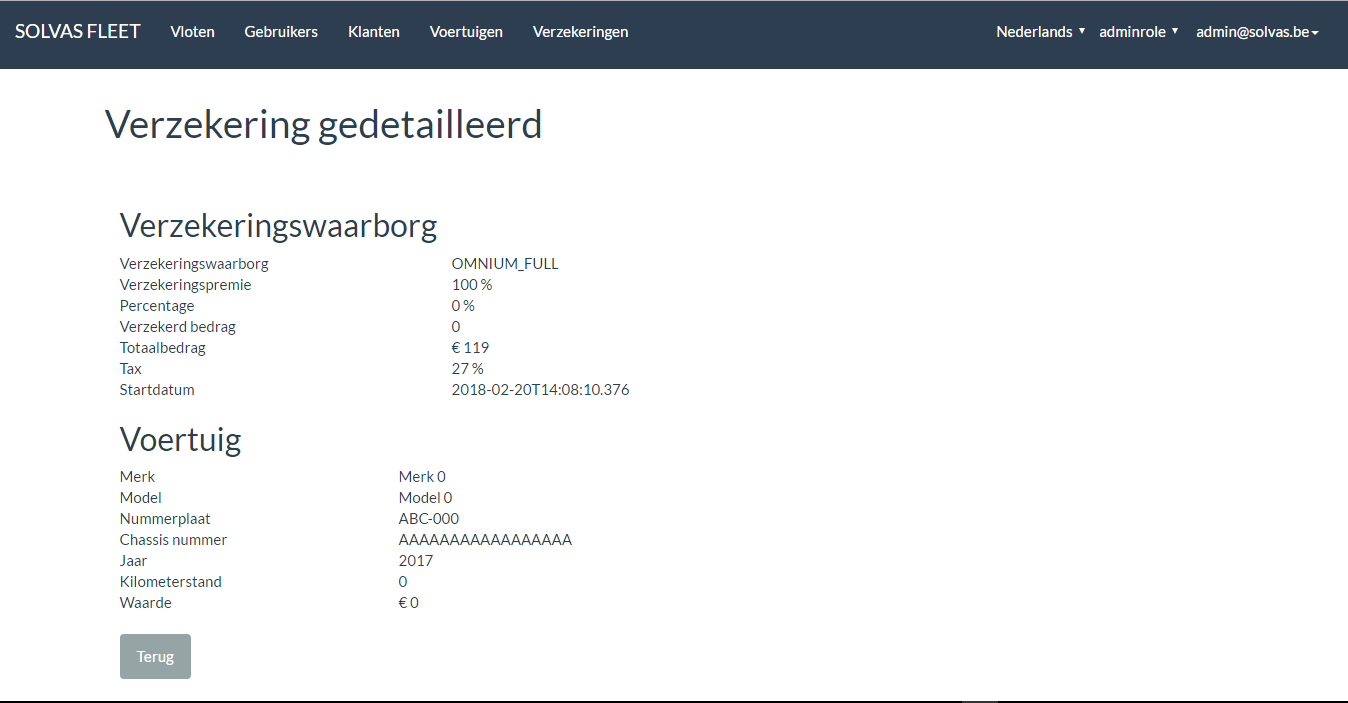
\includegraphics[width=0.9\textwidth]{img/fig_r.png}
	\caption{Bekijken verzekeringswaarborg}
\end{figure}

\end{document}